\chapter{Design and architecture}
% Intro per chapter, refer to problem definition each time, where are we now, what now (for reader)
% Why this chapter
% Paragraphs
% Conclusion of contents of this chapter
% Link to next chapter

We now present a design to address the challenges and utilize the opportunities of working on a mobile device as put forward in the previous chapter.
First in terms of functionality and other requirements, second the overall system architecture.

% now we move Tribler to mobile, so... we need these:

\section{Design principles}
Previous attempts at designing a mobile version of Tribler failed to properly separate re-usable components.
This resulted in unmaintainable code and increased difficulty in testing.
We use a top down approach to come to a high level system architecture and in determining the reusable components or the current Tribler code.
% What is the gap?
Some functionality of Tribler has been shown to work on Android before.
Our design will fill in the gap of connecting the pieces of the grand puzzle to make Tribler fully work on mobile.

% Divide and conquer
Recent refactoring of the Tribler code has divided functionality into core modules.
% Increase cohesion where possible
% Reduce coupling where possible
The purpose of this was to increase cohesion inside modules and the core, and reduce coupling between modules where possible.
This makes porting the core and individual modules easier.
% Increase re-usability where possible
Our design also attempts to maximize re-use-ability with separation of components and clearly defined interfaces.
An API between front-end and back-end is the industry standard of choice here.
% Reuse existing designs and code where possible
% What are the existing modules we re-use?
Having separated the GUI from the back-end, we can easily re-use the Tribler core and ditch the outdated wxPython GUI.
The new GUI can concentrate on Android and smart-phone user interaction.
% Keep the level of abstraction as high as possible
Many established best practices, like Google's "material design", and support libraries that abstract from platform specifics can be re-used.
% reuse of expertise
% reuse of standard designs and algorithms
% reuse of libraries of classes or procedures, of of powerful commands built into languages and operating systems
% reuse of frameworks
% reuse of complete applications
Instead of re-implementing multi-media functionality and player interface, we should re-use an existing library or preferably an entire app.
% Design for flexibility / adaptability
The flexibility of the design benefits from cohesive components with a clearly defined role.
For example: being able to swap out components like the GUI makes Tribler much more adaptable to various mobile devices that may or may not have a display.
The configuration of Tribler core is stored separately from the data and can be altered externally by users since it is saved in a human readable form.
% Anticipate obsolescence
% niet echt iets mee gedaan

% Design for portability
All functionality of Tribler must be packaged in a single installable container.
% Design for testability
The GUI must be able to be tested separately from the back-end and vice-versa.
Also the API must be able to be tested independently and be clearly documented for other developers.

% Design defensively
All Android intents should be explicit. \cite{paper Analysing inter-application communication in Android}
Expose / Export only Android activities and services that should be public

% Availability and resilience
A distinction must be made between user input error and internal exceptions.
The user must be given a chance to correct the input without starting over.
If Tribler crashes it should resume normal operation by just restarting it and optionally ask the user to do so.
% Internationalization
The GUI should support other languages to be added without changing source code.
% Resource usage
The separation of front-end and back-end should not lead to resources being loaded into memory twice or anything of that matter.
% Usability
Make use of universally recognizable icons that are native to the platform UI.
The responsiveness of the GUI must not be significantly impacted by the amount of data presented on screen.
The responsiveness of the GUI must also not be significantly impacted by the amount of computational work, or otherwise, done in the background.


\section{Functional requirements}
% Functional level
% Function design
%Product design involves determining the objectives of the system. Central questions in this process are “what is feasible?”, “what is required?” and “what functions need to be fulfilled by the system?” It is a strategic decision process and it will be termed the function design 
%Function design distinguishes between innovation and improvement. Improvement usually only concerns the reorganisation or reengineering of an existing system, which implies a rearrangement of existing functions or a different interpretation of these functions. Innovation concerns the extension, reduction or modification of functions due to the introduction of new technology, resources and/or organisation.

inputs, commands and conditions
outputs, conditions
store, reuse data, backup
computations
timing and synchronization


Functional requirements

Live production (screenshots) and dissemination
Record video
Create My Channel
Add to My Channel
Search results

MultiChain

Start quickly / delay

REST HTTP JSON API

GUI

Nosetests CI


All functionality of Tribler must be usable directly from the mobile device, without the need or support for any other external device.

Because of the ubiquity of smart-phones with built-in camera one is always at hand and ready to record.
Such mobile devices are much more manageable than for example laptops with built-in camera that Tribler has been capable of running on in the past.
No opportunity has to be missed due to hassle of getting a dedicated camera and transferring the recording to a connectible device afterwards.
Therefore the camera built-in the mobile device should be used to record video or photographs with Tribler.
The usability of Tribler as a content generating tool is greatly improved by this. 

Publishing content should be one simple step for the user to perform, especially right after creating new content.
Every user must be able create his/her own channel in Tribler to publish their content, just like channels in YouTube, directly from the mobile device.
Newly discovered channels and content may be added to the GUI without user interaction.

To easily share your own channel with others the id could be transferred via NFC from device to device.
With just one-click-confirmation it should be send, and the receiving device must then be able to subscribe to this channel and start discovering the contents automatically right away.
Because this may require both devices having Tribler installed, it also must be able to share the installation package via Bluetooth or WiFi without any prerequisites on the receiving device.

Self-created content must be stored on the internal memory and processed automatically on the mobile device itself in order to avoid dependency any external processing unit.
This includes the creation of .torrent files required to share content via the bit-torrent protocol.



impliceert: gewoon opschrijven: 2 processes means communication: impliceert API

%TODO: kijk naar wat in DRAFT staat, dat zijn key dingen



\section{Non-functional requirements}


\subsection{Quality requirements}


All processing tasks should be performed in the background, so as to allow the user to continue working with Tribler or otherwise, while indicating about ongoing processing.
The GUI must be responsive to the users' input at all times, even if the amount of data shown on screen is very large.

If an error occurs that is recoverable the app should automatically retry or ask the user to correct the input if applicable.

To keep the project maintainable the entire build tool-chain must be integrated in the continuous integration and build server of Tribler.
All existing tests should also be performed on Android, with modifications for platform specific tests.
Also all unit tests and integration tests must cover as much code as possible and should be executed on every build.


responsivitity through separation of front and backend


non-bloated

alleen key dingen hiervan:

response time
throughput
resource usage
reliability
availability
recover from failure
maintainability and enhancement
re-usability

\subsection{Platform requirements}

computing platform: min. system specs and features, api level
technology to be used: programming language, db

The minimum API level of Android should support WiFi, Bluetooth and NFC features.



\subsection{Process requirements}

development process / methodology
cost
delivery date




(instant) search





\section{System architecture}
% Design level

systeemdiagram

\begin{figure}[h]
	\centering
	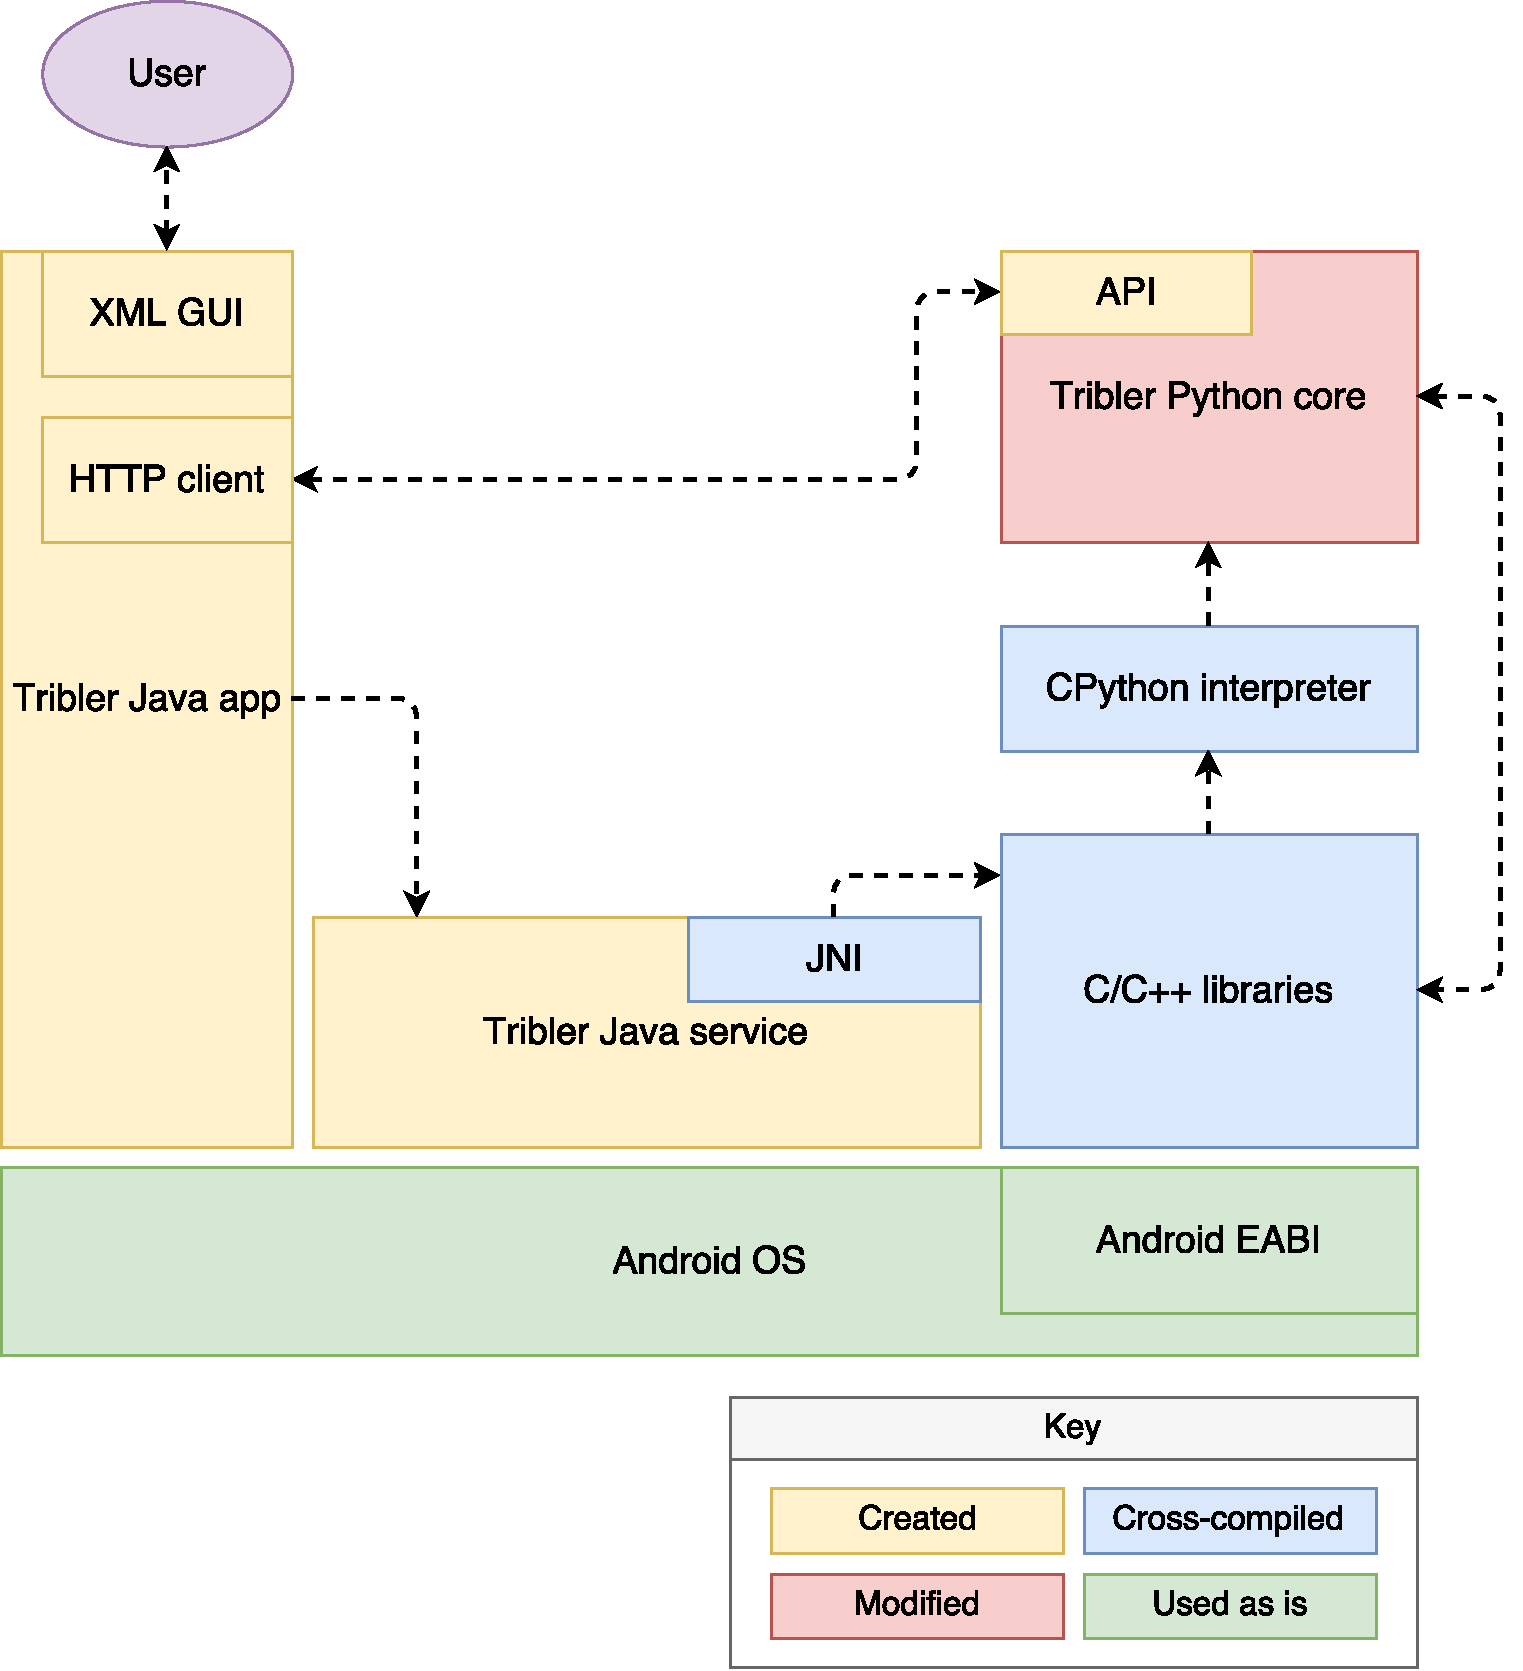
\includegraphics[width=\textwidth]{system_architecture}
	\caption{System architecture}
	\label{fig:system_architecture}
\end{figure}


Previous attempts at creating an Android version of Tribler failed with regards to maintainability.
Poor separation of front-end and back-end meant re-use of the core modules was hard to maintain.
The new architecture clearly separates tasks of the GUI and background operations.


